\chapter{System Design and Implementation}

This chapter describes of the system. It starts by providing overview of the system, followed by requirement elicitation to build prototype. Furthermore, it also provide deeper understanding of architectural paradigm by discussing each module and their interconnection.

\section{Overview}

Pervious chapter limits our discussion about the design decision and describe the essential component of the system.  Since the concept is quite abstract and does not dictate any implementation details.  In order to challenge the relevance and capability of the concept, a prototype app, tailored to a real world scenario, should be developed as a “proof of concept”. Our system is divided in to two components: (1) Rest based web application follows modular principle of system design i.e. functionality of a system is divided into multiple concurrent modules. Where coordination of modules depend on database.  Each module has its own Data Access Object (DAO) through with communication take place. Module query existing data with the help of DAO perform their task and update afterward. (2) iOS client provides all the required interface to communicate with the server. It aims to collect information that needs to build user profile and allow active learning and critiquing mechanism to update user profile and increase the trust between user and system by conveying the idea how much system cares about user and his need. 

\section{Requirment elicitation}

This section represents user’s viewpoint of the system. It also describes the purpose of the system by identifying the Functional, non-functional requirements and description of use case in the form of scenarios. It is important to mention here that all the scenarios are developed to evaluate the prototype and are not meant for production purpose. 

\subsection{Functional Requirments}

FoodForMe is a mobile food recommender system that user iOS platform. It purpose to facilitate user to find the food what to cook that matches their personal preferences. Idea behind this prototype application is to proof the concept a combination of Persuasion and critique-based recommender system lead to better recommender and have an impact on user decision making process. Therefore all the functionality in a design is bounded to this purpose. There are two cases of interaction with the system. In case one user need login via Facebook so that system can get its demographic profile instead of asking him to fill out his personal information. Demographic information contains name, birthday, email, name and link of his profile picture. By default system keeps his cooking time preference and course selection preference. User can change these preferences from the setting screen. In second case user can interact without login and having same default preference. As it is notice that some user hesitate to provide their information without having a trust in a system. However, in this particular case user can only view the information. Our rest of discussion will relate do case one.\newline

After getting login and change his preference. User will able to view recipes according to his preference. Each recipe shows the name, star rating, main categories, sub categories, number of reviews and recipe picture. Once the user tap on any recipe, user is able to view detail of selected recipe. Detail screen consists on 3 to 4 sections depends on screen type. Section 1 contains the generic information about the recipe same as discuss above accept it provide large Image of recipe. In Section 2 is related to recipe ingredients, each ingredient item have its name and quantity. Section 3 is about preparation/direction means its guide user how to cook that recipe. Section 4 is an option selection and it will appear as per screen type. In this section system will provide why system think this recipe is according to user preference. User is able to see two screens that display recipes list. First one will display the popular recipes of the system. Recipe course and popularity are the factors on which this will depends on. Motivation behind this to aware user what’s new and hot in system and allow user to change his taste. On the other hand second list will depends only user preference. On detail screen of each recipe system will provide explanation, which tells user what system will think about him and why these recipe recommend to him. \newline

On the detail screen of selected recipe user can criticized on showed item. User can critique on list of indigents by mentioning them he like that ingredient or not. Also he might be able to critique on recipe by given star according to his choice. Additional system allow user to change his personal preferences these include cooking time and course selection. \newline


\subsection{Non Requirments}

From usability to performance aspect of a system Non-functional requirement can apply in many ways. However it is our assumption that this app is a prototype and will only use for evaluation purpose but we have to consider User interface, performance and supportable requirements \cite{burigat2005bringing}. Following are some few non-functional requirements that should guide to development process:

\begin{enumerate}

	\item App must not be crash.
	\item Any mobile user can use the application and have a clear understanding of app without facing any problem.
	\item App should provide consistence user interface with respect to colors, fonts and theme.
	\item App should follow the Application User interface guideline provided by apple.
	\item For app start to critiquing or selection of preference must be reachable at any time.
	\item Processing time of app may not exceed to 1 second. 
	\item Server calls should not take more 30 sec.

\end{enumerate}

\subsection{Use-Cases}

Figure \ref{fig:ch4_use_case_foodforme} illustrates foodforme uses cases.  These include importing of user demographic information via Facebook, logout user form applicaiton, user can change his preference according to his convenience, browsing of recipes, critiquing on recipe based on ingredients and rating and selection of recipe to cook. To discuss the use cases we follow the scenario based approach. \cite{bruegge2004object}.

\begin{figure}[h]
	\centering
	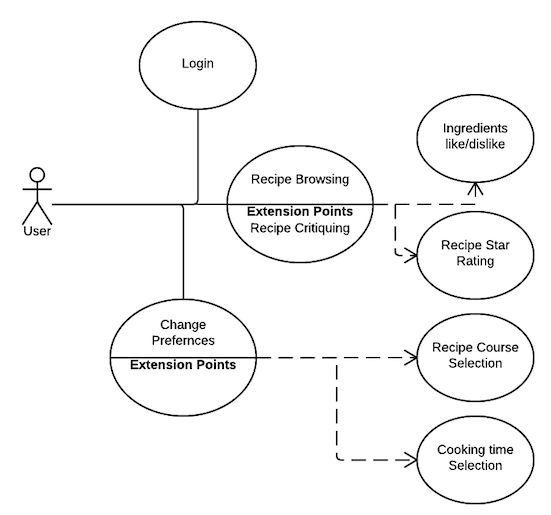
\includegraphics[width=.5\linewidth]{figures/ch4_use_case_foodforme.png}
	\caption{FoodForMe use case diagram}
	\label{fig:ch4_use_case_foodforme}
\end{figure}

\newpage
 
 The first use case, determine user login via Facebook to get his Facebook profile to avoid filling his demographic information by his own. Login flow should provide good user experience and follows the standard practices. Use case start any point of time after app launch and user click on main menu and ends once user can see his name and profile picture at menu screen.  Table \ref{table:import_user-demographic-information} provides the scenario description. \newline
 
 \begin{table}[ht]
 	\centering % used for centering table
 	\begin{tabular}{p{4cm} p{10cm}}  % centered columns (4 columns)
 		\hline\hline %inserts double horizontal lines
 		Use case name & Determine stereotype \\ % inserts table
 		%heading
 		\hline % inserts single horizontal line
 		
		Participating actor & Initiated by User \\ % inserting body of the table
 		Flow of events & (1). User starts app.
 		(2). Click on menu button.
	 	(3). Tap on login via Facebook button to import his Facebook profile. \\
 		Entry condition & User starts app\\
 		Exit condition & User can see his Facebook profile image and name on application slide menu.\\
 		Quality requirements & (1) Import user profile via Facebook SDK. (2) Profile should be import in one click excluding of Facebook login process. (3) It should take more than 30 seconds.\\ [1ex] % [1ex] adds vertical space
 		\hline %inserts single line
 	\end{tabular}
 	\caption{Use case 1:Import user demographic information}
 	\label{table:import_user-demographic-information}
 \end{table}
 
 The second use case, application allow user to logout from application by providing standard mechanism provided by Facebook. After login he is not able to see his personal information in app. Table \ref{table:user_logout} determines the event flow.
  
  \begin{table}[ht]
  	\centering % used for centering table
  	\begin{tabular}{p{4cm} p{10cm}}  % centered columns (4 columns)
  		\hline\hline %inserts double horizontal lines
  		Use case name & Determine stereotype \\ % inserts table
  		%heading
  		\hline % inserts single horizontal line
  		
  		Participating actor & Initiated by User \\ % inserting body of the table
  		Flow of events & 1. User starts app.\newline
  		2. Click on menu button.\newline
  		3. Tap on logout via Facebook button to logout his Facebook profile.\newline
  		4. App shows logout confirmation which includes logout and cancle \\
  		Entry condition & User starts app\\
  		Exit condition & User can logout form applicaiton and unable to his profile picture and name on app menu.\\
  		Quality requirements & 1. User able to logout from system in two clicks.\newline
  		2. It should take more than 30 seconds.\\ [1ex] % [1ex] adds vertical space
  		\hline %inserts single line
  	\end{tabular}
  	\caption{Use case 2: Logout use}
  	\label{table:user_logout}
  \end{table}
 
 Table\ref{table:recipe_browsing} describe use case regarding recipe browsing. According to this user can browse the recipes list that is recommended to him by scrolling up and down. Where recipe list have star rating, recipe name, recipe’s category, review count of recipe.
 
   \begin{table}[ht]
   	\centering % used for centering table
   	\begin{tabular}{p{4cm} p{10cm}}  % centered columns (4 columns)
   		\hline\hline %inserts double horizontal lines
   		Use case name & Determine stereotype \\ % inserts table
   		%heading
   		\hline % inserts single horizontal line
   		
   		Participating actor & Initiated by User \\ % inserting body of the table
   		Flow of events & 1. User can tap on popular/ recommend recipes view.\newline 
   		2. User can see the list of recipes.\newline
   		3. User can perform scrolling to view more recipes.\\
   		Entry condition & User starts app\\
   		Exit condition & User can found his favorite recipe to cook.\\
   		Quality requirements & 1. Scrolling of recipes should be sleek.
   		2. Each item should have name, star rating, avatar or recipe, review count and primary catagory.\\ [1ex] % [1ex] adds vertical space
   		\hline %inserts single line
   	\end{tabular}
   	\caption{Use case 3: Recipe browsing}
   	\label{table:recipe_browsing}
   \end{table}
   
Use case 4 is regarding the showing the detail of selected recipe. This use case is depended use case 3.  On detail screen user can view large image of recipe including all the parameters that is use case 3. Moreover it should display the ingredients along with their quantity. Finally it displays preparation method means how to cook that recipe. Senerios is describe in Table\ref{table:recipe_detail}
   \begin{table}[ht]
   	\centering % used for centering table
   	\begin{tabular}{p{4cm} p{10cm}}  % centered columns (4 columns)
   		\hline\hline %inserts double horizontal lines
   		Use case name & Determine stereotype \\ % inserts table
   		%heading
   		\hline % inserts single horizontal line
   		
   		Participating actor & Initiated by User \\ % inserting body of the table
   		Flow of events & 1. User selects recipe from list (Use case 3)\newline 
   		2. User can see ingredients of selected recipe along with quantity.\newline
   		3. User can cooking method\\
   		Entry condition & User select a recipe from recommended item\\
   		Exit condition & User can found his favorite recipe to cook.\\
   		Quality requirements & 1. Scrolling of recipe should be sleek. 2. Each item should have cooking method and set of ingredients along with quantity\\ [1ex] % [1ex] adds vertical space
   		\hline %inserts single line
   	\end{tabular}
   	\caption{Use case 4: Recipe Detail}
   	\label{table:recipe_detail}
   \end{table}
   
   Use case 5 of our system is critiquing a recipe. System allows user to critique on user’s recommend recipe so that system will aware about user taste and his health need. In our system critiquing of recipe and its ingredient is down by separately so that we can evaluate user taste more specifically. It might be possible that user doesn’t like the recipe but his likes the ingredient and those ingredients are the essential one for his dietary need. Therefore, recipe critiquing is done via star rating where ingredient can be critique by like/dislike. Table \ref{table:recipe_ingredient_critique} discuss the event flow of this use case.
   
   
    \begin{table}[ht]
    	\centering % used for centering table
    	\begin{tabular}{p{4cm} p{10cm}}  % centered columns (4 columns)
    		\hline\hline %inserts double horizontal lines
    		Use case name & Determine stereotype \\ % inserts table
    		%heading
    		\hline % inserts single horizontal line
    		
    		Participating actor & Initiated by User \\ % inserting body of the table
    		Flow of events & 1. User is viewing recipe detail 
			He wants to give his feed back about recommend recipe. 
			2. He taps on Critique button at top right corner of recipe detail screen. 
			3. On critique screen he may like/dislike ingredients. 
			4. He may rate recipe by selecting stars.\\
    		Entry condition & use case 1, 3, 4\\
    		Exit condition & User can found his favorite recipe to cook.\\
    		Quality requirements & 1. Like/dislike have differnt color 2. Rating of recipe is done via stars selection\\ [1ex] % [1ex] adds vertical space
    		\hline %inserts single line
    	\end{tabular}
    	\caption{Use case 5: Recipe Critique}
    	\label{table:recipe_ingredient_critique}
    \end{table}
    
    
\section{User interface}    

Current section focuses on the implementation of user interface of application, FoodForMe, It is our fundamental requirement to build a high fidelity prototype that will run iOS platform and supported device should be iPhone. Current implementation of prototype will run on iOS 8.3 and above. Last year 2014, when apple announced iOS 8 they introduced a new programing language for developing iOS application called “swift”. They also declared that objective-c will not going to be obsolete. Therefore we have a choice to select the preferred language for developing client. We chose swift for our development. Reason behind selecting a Swift over objective-c is swift is 1.3x faster then objective which have an impact on performance factor of our app. Swift also provide many features like closures and etc. which is legged by objective-c.  Application UI was designed with the help of Storyboard technique.  The entire user interface of application is based on Auto Layout Guideline provided by Apple Inc. Auto layout is a system that helps in developing UI by creating a mathematical description of the relationships between the elements. To achieve the persuasion effect it is very important to focus each and every element of UI. Later in this section we discuss each screen implement and behavior of application. Finally section will close by discussing the data model for app.

\subsection{Main Menu}

FoodForMe main menu allows user to perform navigation inside the application from one screen to another screen. These screens include Popular recopies, Recommendations and Preferences. It is also responsible for representing user login status.  Categorically we have two modes and refer as “User Logout Mode” and “User Login Mode”. Each mode has in settings value in terms of presentation and behavior of application. Initially app starts with  “User Logout Mode” in this status. In this mode app will show “Login Via Facebook” at the bottom of the menu along with default avatar on the top of the menu as show in Figure\ref{foodforme_main_menu_screen_logout}. Once user click on “Login Via Facebook” and successfully login then app will enter in second mode i.e. display his Name, Avatar and lower button will change to “Logout” as shown is Figure\ref{foodforme_main_menu_screen_logout}. These modes have impact on application interaction cycle. The idea behind introducing two modes is to allow user to have a glance of app without force him login. Once he is comfortable with the app and he trust the app then he can perform login. After login application will provide personalized information that is based on user interest. Second and importantly Login via facebook is one of the common and the quickest method to gather the user demographic information.

\begin{figure}[h]
	\begin{subfigure}{.49\textwidth}
		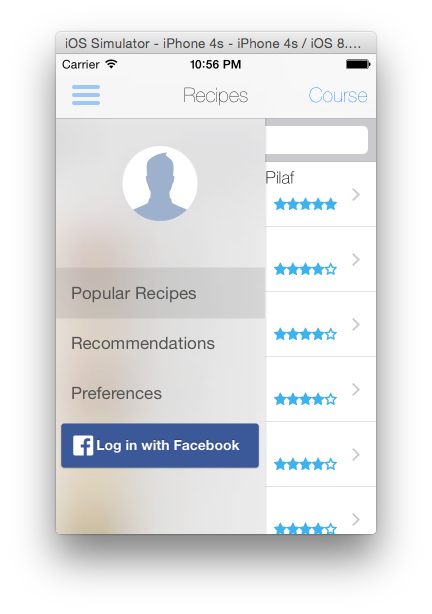
\includegraphics[width=.9\linewidth]{figures/ch4_app_screen_shots/main_menu/main_menu_1.png}
		\caption{Logout user}
	   \label{foodforme_main_menu_screen_logout}
	\end{subfigure}
	\begin{subfigure}{.49\textwidth}
		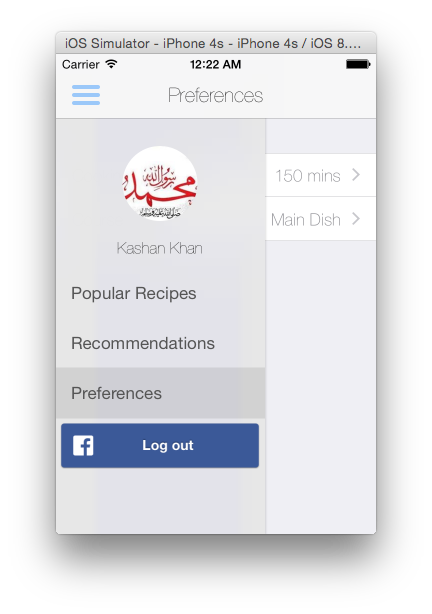
\includegraphics[width=.9\linewidth]{figures/ch4_app_screen_shots/main_menu/main_menu_2.png}
		\caption{Login user}
		\label{foodforme_main_menu_screen_login}
	\end{subfigure}
	\caption{FoodForMe Main Menu}
	\label{fig:foodforme_main_menu_screen}
\end{figure}
	  
\subsection{Popular/Recommended Recipes}

Popular and Recommended Recipes are the two important interfaces of our app which looks a like to each other but have slightly different functionality between them. Figure\ref{fig:foodforme_recipe_screen} is representation how it look likes. We put more attention in design phase and tried our best to follow the user-centric design approach.  Also finding out the primary factors that will help in structure of recipes to increase and mentation user’s interest to achieve transparency, efficiency, effectiveness and satisfaction. To achieve this we display recipe name, rating, category, subcategory of recipe, recipe’s avatar and sort of recipe by tile. However all recipes that are recommended to user is based on his preferences and course selection. Considering the fact that user can change his course any time therefore we provide course button at the top right corner to change his course.

 \begin{figure}[h]
 	\centering
	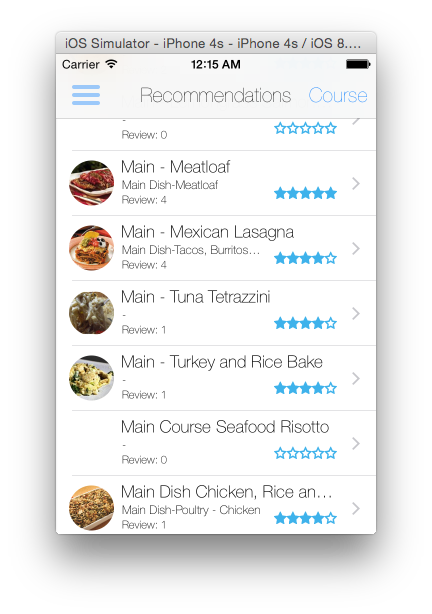
\includegraphics[width=.5\linewidth]{figures/ch4_app_screen_shots/recipes/recipes.png}
    \caption{FoodForMe Recipes List}
	\label{fig:foodforme_recipe_screen}
	\end{figure}
	  
\subsection{Recipe Detail} 

Design of recipe detail follows conventional layout practices. These include by providing recipe information at the top with large avatar, ingredients along with quantity and last but not the least preparation description that helps to cook that recipes. Figure\ref{fig:foodforme_recipe_detail_screens} is the visual representation of interface. Keeping in mind that user can critique on recipe and it’s ingredient therefore critique button is added to top of screen. 
	  \begin{figure}[h]
	  	\begin{subfigure}{.32\textwidth}
	  		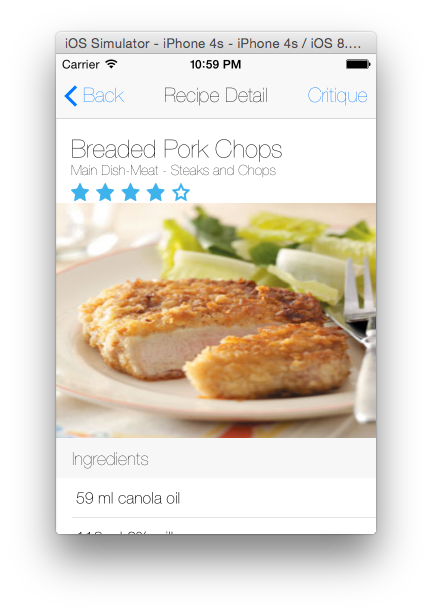
\includegraphics[width=.9\linewidth]{figures/ch4_app_screen_shots/recipe_detail/recipe_detail_1.png}
	  		\caption{Recipe Header}
	  	\end{subfigure}
	  	\begin{subfigure}{.32\textwidth}
	  		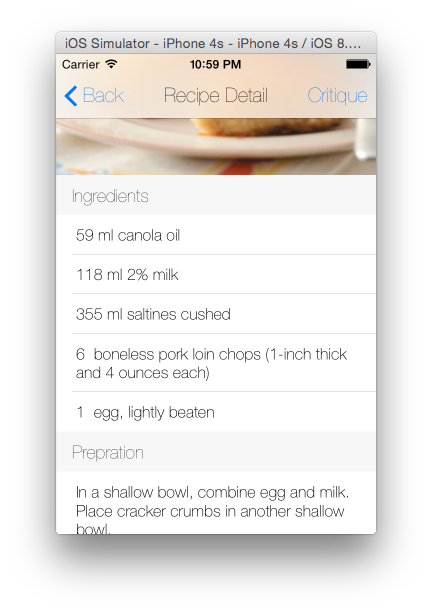
\includegraphics[width=.9\linewidth]{figures/ch4_app_screen_shots/recipe_detail/recipe_detail_2.png}
	  		\caption{Recipe's Ingredients}
	  	\end{subfigure}
	  	\begin{subfigure}{.32\textwidth}
	  		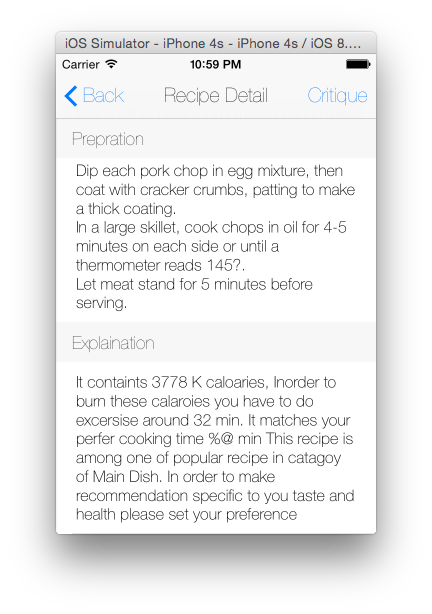
\includegraphics[width=.9\linewidth]{figures/ch4_app_screen_shots/recipe_detail/recipe_detail_3.png}
	  		\caption{Recipe Preparation}
		  	\end{subfigure}
	  	\caption{FoodForMe Recipe Detail}
	  	\label{fig:foodforme_recipe_detail_screens}
	  \end{figure}

\newpage
\subsubsection{Recipe's Explanation}

Earlier in this section we discussed that Recommended and Popular recipes have same interface but the difference comes in recipe detail. Popular recipes do not requires any information, as is task to get the knowledge about user by providing him diverse result. However, Recommend recipes should always provide explanation about why system thinks this recipe is suitable for user along with two additional factors i.e. calories and exercise time needs to burn such calories. Where, determination of suitability is integration of course selection, user preferred cooking and his taste and health preferences. Additionally system provides two types of explanations depending on user login status. If user is offline or logout, in explanation system tries to motivate user to login to get accurate recipe according to him. Figure\ref{fig:foodforme_recipe_explanation} shows the FoodForMe recipe's explanation.  


\begin{figure}[h]
	\begin{subfigure}{.49\textwidth}
		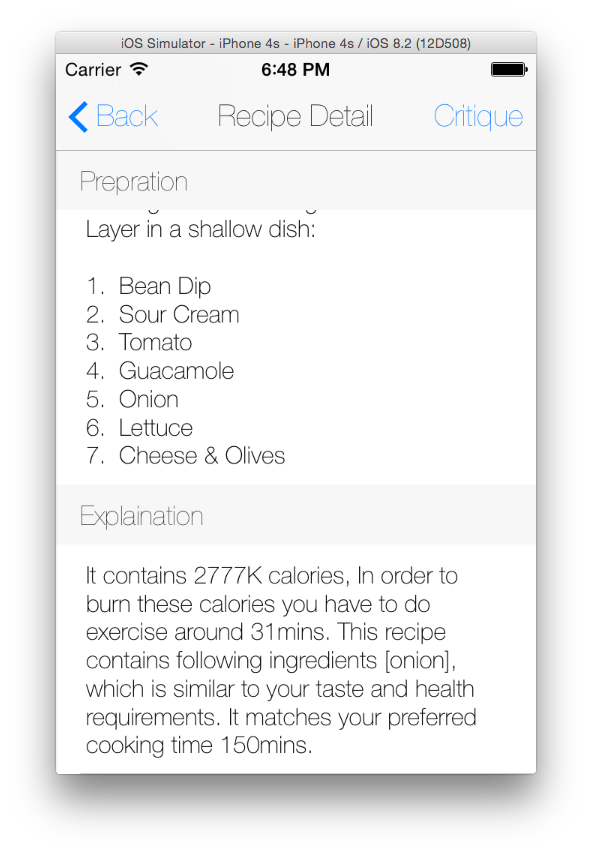
\includegraphics[width=.9\linewidth]{figures/ch4_app_screen_shots/recipe_detail/recommended_recipe_explaination/recommended_recipe_explaination_2.png}
		\caption{Recipe's explanation For Logout user}
		\label{fig:foodforme_recipe_explanation_2}
	\end{subfigure}
	\begin{subfigure}{.49\textwidth}
		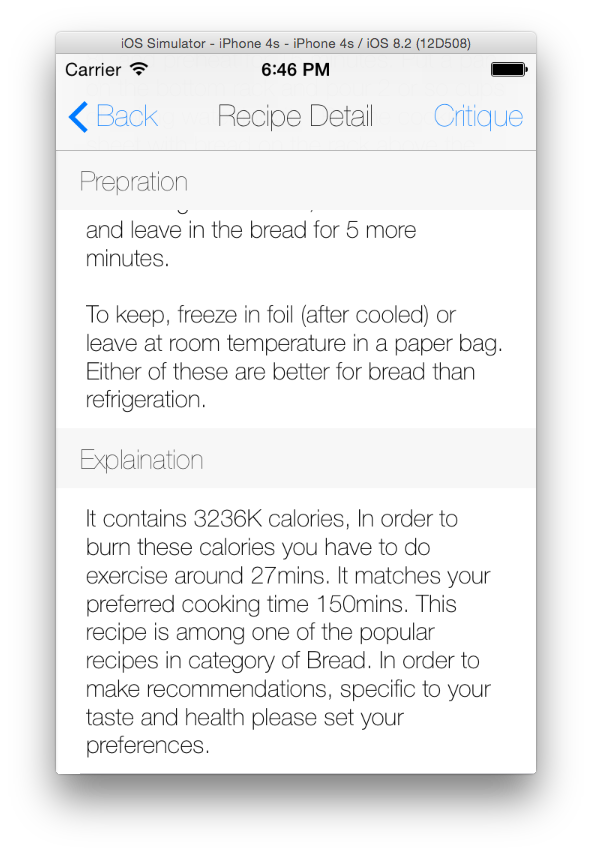
\includegraphics[width=.9\linewidth]{figures/ch4_app_screen_shots/recipe_detail/recommended_recipe_explaination/recommended_recipe_explaination_1.png}
		\caption{Recipe's explanation For Login user}
		\label{fig:foodforme_recipe_explanation_1}
	\end{subfigure}
	\caption{FoodForMe Recipe Explanation}
	\label{fig:foodforme_recipe_explanation}
\end{figure}

\subsection{Recipe critiquing} 
For Personalize recommender system is a important to know user preferences. More knowledge about the user more accurate the recommendations are. Critiquing recipes allow us to determine the user interests in our system. Focusing on critiquing importance our design should be intuitive, interactive and helps user to perform critiquing fast enough. Our assumption was user may not like some recipes but ingredients in that recipe have an impact on preference. Also it is important to what accent user likes or dislikes the recipe. Therefore we separated recipe and ingredients critiquing. Star rating is preferable for recipe critique. As far as ingredients critique concerns it should be like or dislike. While our implement of this screen have separated into 3 sections. Top one was about the recipe information, Middle deals with ingredients and Last section is about given stars to recipe to selected recipe.  Since the critiquing of ingredients is Boolean in nature so we can use default UISwitch presents on iOS sdk but they are not much intuitive nature and may confuse users. Thus, our design follows the simple toggling button which red and green color for liking and disliking ingredients. Figure\ref{fig:foodforme_recpie_critiquing} show how we implemented this screen.


	  \begin{figure}[h]
	  	\begin{subfigure}{.32\textwidth}
	  		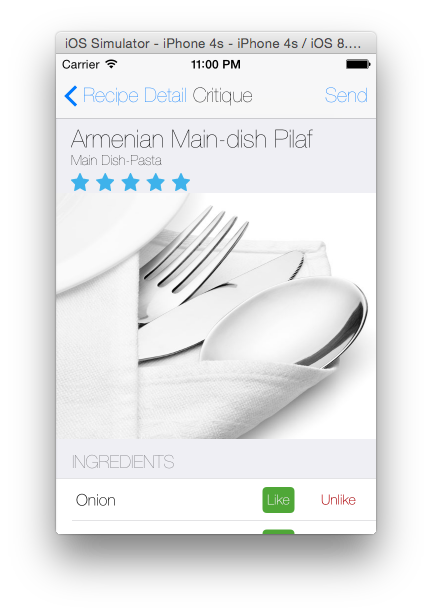
\includegraphics[width=.9\linewidth]{figures/ch4_app_screen_shots/critique/critique_1.png}
	  		\caption{Recipe Header}
	  	\end{subfigure}
	  	\begin{subfigure}{.32\textwidth}
	  		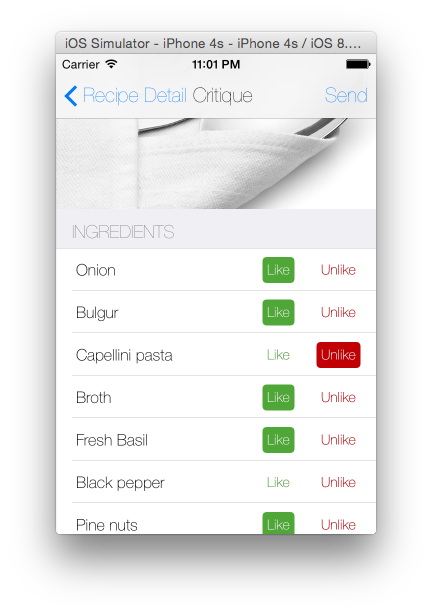
\includegraphics[width=.9\linewidth]{figures/ch4_app_screen_shots/critique/critique_2.png}
	  		\caption{Ingredents Critique}
	  	\end{subfigure}
	  	\begin{subfigure}{.32\textwidth}
	  		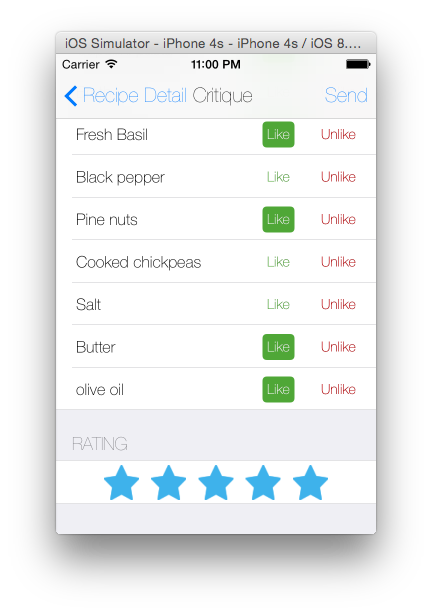
\includegraphics[width=.9\linewidth]{figures/ch4_app_screen_shots/critique/critique_4.png}
	  		\caption{Recipe's Critique}
	  		\end{subfigure}
	  	\caption{FoodForMe Recipe Detail}
	  	\label{fig:foodforme_recpie_critiquing}
	  \end{figure}
\newpage
\subsection{Preferences} 

User context is important aspect to refine recommendations. Cooking time and Course are the two important explicit contexts that our system required from the iOS app.  In our application Preferences screen allow user to select these context according to his choice. After taping on any item a detail screen will appear that allow user to select the value from required list. Figure\ref{fig:foodforme_preferences} shows the implementation of Preferences. 

	  \begin{figure}[h]
	  	\begin{subfigure}{.32\textwidth}
	  		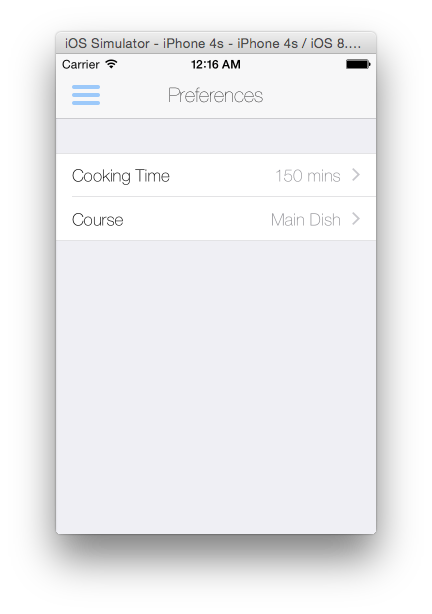
\includegraphics[width=.75\linewidth]{figures/ch4_app_screen_shots/preferences/peferences.png}
	  		\caption{General Peferences}
	  		%\label{fig:ch2_lamche2014active_1}
	  	\end{subfigure}
	  	\begin{subfigure}{.32\textwidth}
	  		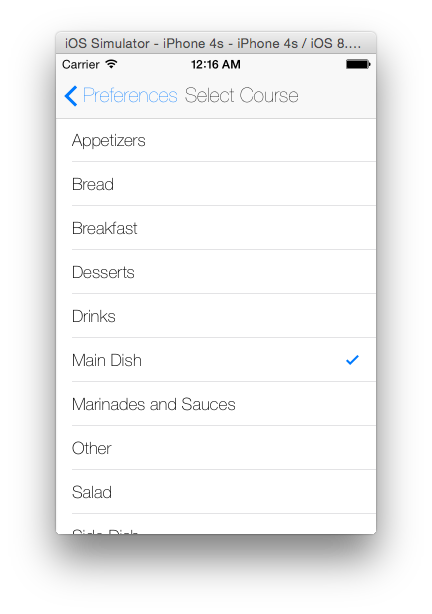
\includegraphics[width=.75\linewidth]{figures/ch4_app_screen_shots/preferences/peferences_course.png}
	  		\caption{Recipe's Course Selection}
	  		%\label{fig:ch2_lamche2014active_2}
	  	\end{subfigure}
	  	\begin{subfigure}{.32\textwidth}
	  		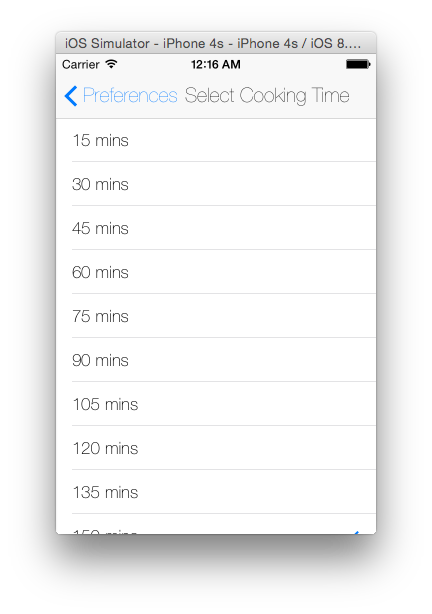
\includegraphics[width=.75\linewidth]{figures/ch4_app_screen_shots/preferences/peferences_cooking_time.png}
	  		\caption{Cooking Time Selection}
	  		%\label{fig:ch2_lamche2014active_2}
	  	\end{subfigure}
	  	\caption{FoodForMe Recipe Detail}
	  	\label{fig:foodforme_preferences}
	  \end{figure}
	  
\newpage
\subsection{iOS Data Model}	  


	   \begin{figure}[h]
	   	\centering
	   	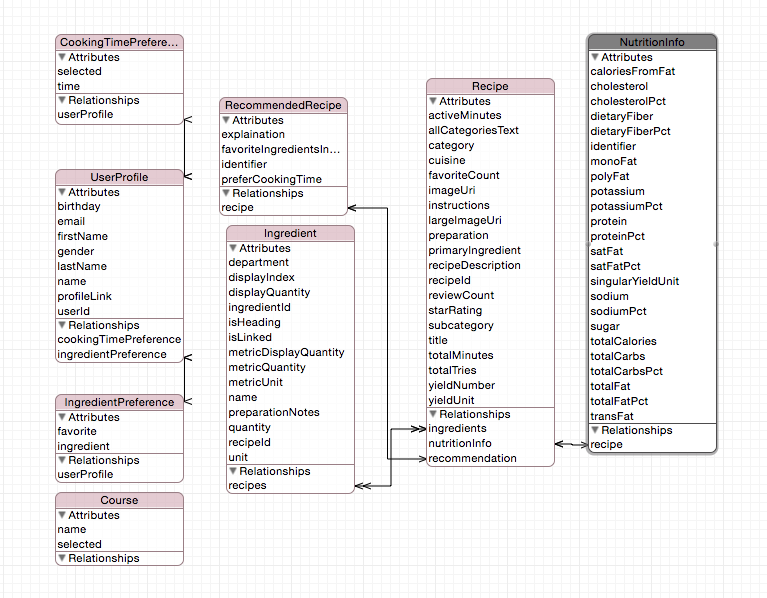
\includegraphics[width=1\linewidth]{figures/ch4_ios_data_model}
	   	\caption{FoodForMe iOS Data Model}
	   	\label{fig:foodforme_ios_data_model}
	   \end{figure}
	   
	  
	  
\section{System Architecture}

\subsection{Working}

\subsection{Class Drigram}

\subsection{ERD}

\section{System Services}

\subsection{Service 1}
